\documentclass{beamer}
\beamertemplatenavigationsymbolsempty

\usepackage[utf8]{inputenc}
\usepackage[ngerman]{babel}
\usepackage{graphicx}
\usepackage{pdfpages}
\usepackage{hyperref}

\title{Fachschaft Informatik}

\begin{document}
	\maketitle

	\begin{frame}{Warum fsi?}
		\begin{itemize}
			\item Der Verlauf eures Studiums ist bestimmt durch:
				\begin{itemize}
					\item Modulhandbuch
					\item Prüfungsordnung
				\end{itemize}
			\item Wenn etwas schief läuft müsst ihr zum
				\begin{itemize}
					\item Prüfungsamt
					\item Prüfungsausschuss
				\end{itemize}
		\end{itemize}
	\end{frame}

	\begin{frame}{Unsere offiziellen Aufgaben}
		\framesubtitle{Gremienarbeit}
		Wir vertreten euch
		\begin{itemize}
			\item im Fakultätsrat (FakRat)
			\item in den Studienkomissionen (StudKomm)
			\item in den Prüfungsausschüssen (PA)
			\item in der Fachschaftenrätevollversammlung (FSRVV)
			\item ... und in vielen anderen Gremien und Kommissionen
			\item[$\rightarrow$] www.fsi.uni-tuebingen.de/fachschaft/vertreter
		\end{itemize}
		Durch einen ``guten Draht'' zu den Professoren können wir Probleme aufzeigen und gegebenenfalls vermitteln.
	\end{frame}

	% %Nicht in der VL

	% \begin{frame}{Fakultätsrat}
	% 	Entscheidet über
	% 	\begin{itemize}
	% 		\item Finanzen
	% 		\item neue Professuren
	% 		\item Forschung und Lehre
	% 		\item Besetzung von Gremien
	% 	\end{itemize}
	% 	Wird jährlich von allen Studierenden der Fakultät gewählt (5 Studenten aus 11 Fachschaften).
	% \end{frame}

	% \begin{frame}{Studienkommission}
	% 	\begin{itemize}
	% 		\item Wichtigstes Gremium für den Studienablauf
	% 		\item Gestaltet Modulhandbuch
	% 		\item Zwei Kommissionen:
	% 			\begin{itemize}
	% 				\item (Bio-, Medien-, Medizin-) Informatik
	% 				\item Kognitionswissenschaft
	% 			\end{itemize}
	% 		\item 4 Profs, 2 Mitarbeiter, 4 Fachschaftler\\
	% 			$\Rightarrow$ großer Einfluss der fsi
	% 	\end{itemize}
	% \end{frame}

	% \begin{frame}{Prüfungsausschuss}
	% 	\begin{itemize}
	% 		\item Anerkennung von Studienleistungen
	% 			\begin{itemize}
	% 				\item Auslandssemester?
	% 				\item ungewöhnliche Vorlesung für ein bestimmtes Modul?
	% 				\item neues Nebenfach?
	% 			\end{itemize}
	% 		\item (theoretisch) PA für jeden Studiengang einzeln
	% 		\item Fachschaftler mit beratender Stimme
	% 	\end{itemize}
	% \end{frame}

	% \begin{frame}{Hochschulpolitik}
	% 	\begin{itemize}
	% 		\item StuRa - Studierendenrat (ersetzt ASTA)
	% 			\begin{itemize}
	% 				\item Hochschulpolitisches Mandat
	% 				\item kann Projekte unterstützen
	% 				\item Gebühren zu Beginn des Semesters
	% 			\end{itemize}
	% 		\item Senat
	% 		\item Vertreter fühlen sich meist einer Hochschulpolitischen Gruppe zugehörig:
	% 			\begin{itemize}
	% 				\item FSVV
	% 				\item GHG
	% 				\item JuSos
	% 				\item RCDS
	% 				\item ...
	% 			\end{itemize}
	% 	\end{itemize}
	% \end{frame}

	% \begin{frame}{Was wir sonst noch für euch tun}
	% 	\begin{itemize}
	% 		\item Webseite – Zentraler Informationsknotenpunkt
	% 		\item Mailinglisten – Austausch unter den Studenten
	% 		\item Prüfungsprotokolle –\\
	% 			Was fragt ein Prüfer eigentlich so in der Prüfung?\\
	% 			Geschrieben von Studenten für Studenten.
	% 		\item Anfängerbetreuung: Tipps fürs Studium, Frühstück, Kneipentour, Anfängerwochenende,...
	% 		\item Partys und Feste organisieren :-)
	% 	\end{itemize}
	% \end{frame}

	%Nur VL
	\begin{frame}{Was wir sonst noch für euch tun...}
	\framesubtitle{Sommerfest}
		\begin{columns}
			\begin{column}{.5\linewidth}
				\begin{itemize}
					\item einmal im Jahr
					\item immer Ende Juni / Anfang Juli
					\item dieses Jahr 2014-06-27
				\end{itemize}
			\end{column}
			\begin{column}{.5\linewidth}
				Letztes Jahr:\vspace*{2mm}\\
				
\includegraphics[width=\linewidth]{sf13.png}
			\end{column}
		\end{columns}
	\end{frame}

	\begin{frame}{ClubHausFest}
		\begin{columns}
			\begin{column}{.5\linewidth}
				\begin{itemize}
					\item immer donnerstags
					\item zusammen mit der Fachschaft Psychologie
					\item jedes Semester
					\item im Clubhaus
					\item dieses Semester 2014-04-24
				\end{itemize}
			\end{column}
			\begin{column}{.5\linewidth}
				
\includegraphics[width=\linewidth]{CHF_Flyer.png}
			\end{column}
		\end{columns}
	\end{frame}


	% % Nicht in VL
	% \begin{frame}
	% 	\begin{center}
	% 		
\includegraphics[scale=0.45]{CHF_Flyer.png}
	% 	\end{center}
	% \end{frame}


	% \begin{frame}{Sommerfest}
	% 	\begin{columns}
	% 		\begin{column}{.5\linewidth}
	% 			\begin{itemize}
	% 				\item auf dem Sand
	% 				\item Volleyballspiel fsi vs. Profs
	% 				\item jedes Sommersemester (Ende Juni / Anfang Juli)
	% 			\end{itemize}
	% 		\end{column}
	% 		\begin{column}{.5\linewidth}
	% 			
\includegraphics[width=\linewidth]{sf10.png}
	% 		\end{column}
	% 	\end{columns}
	% \end{frame}

	% {\setbeamercolor{background canvas}{bg=black}
	% \begin{frame}
	% 	\begin{center}
	% 		
\includegraphics[height=.95\paperheight]{sf13.png}
	% 	\end{center}
	% \end{frame}
	% }

	\begin{frame}[<+->]{Mailinglisten}
		\begin{itemize}
			\item info-studium
			\item kogwiss
			\item info-jobs
			\item info-talk
			\item info-alumni
			\item Anmeldung:\\
				Mail an \$LISTNAME-subscribe@fsi.uni-tuebingen.de 
		\end{itemize}
	\end{frame}

	\begin{frame}{Fachschaftsarbeit - wie geht das?}
		\begin{columns}
			\begin{column}{.5\linewidth}
				\begin{itemize}
					\item wöchentliche Sitzung im fsi-Zimmer
					\item C125 (Sand Haupteingang - rechts - vor der zweiten Glastür links)
					\item voraussichtlich Donnerstag 18:30 (st)
				\end{itemize}
			\end{column}
			\begin{column}{0.5\linewidth}
				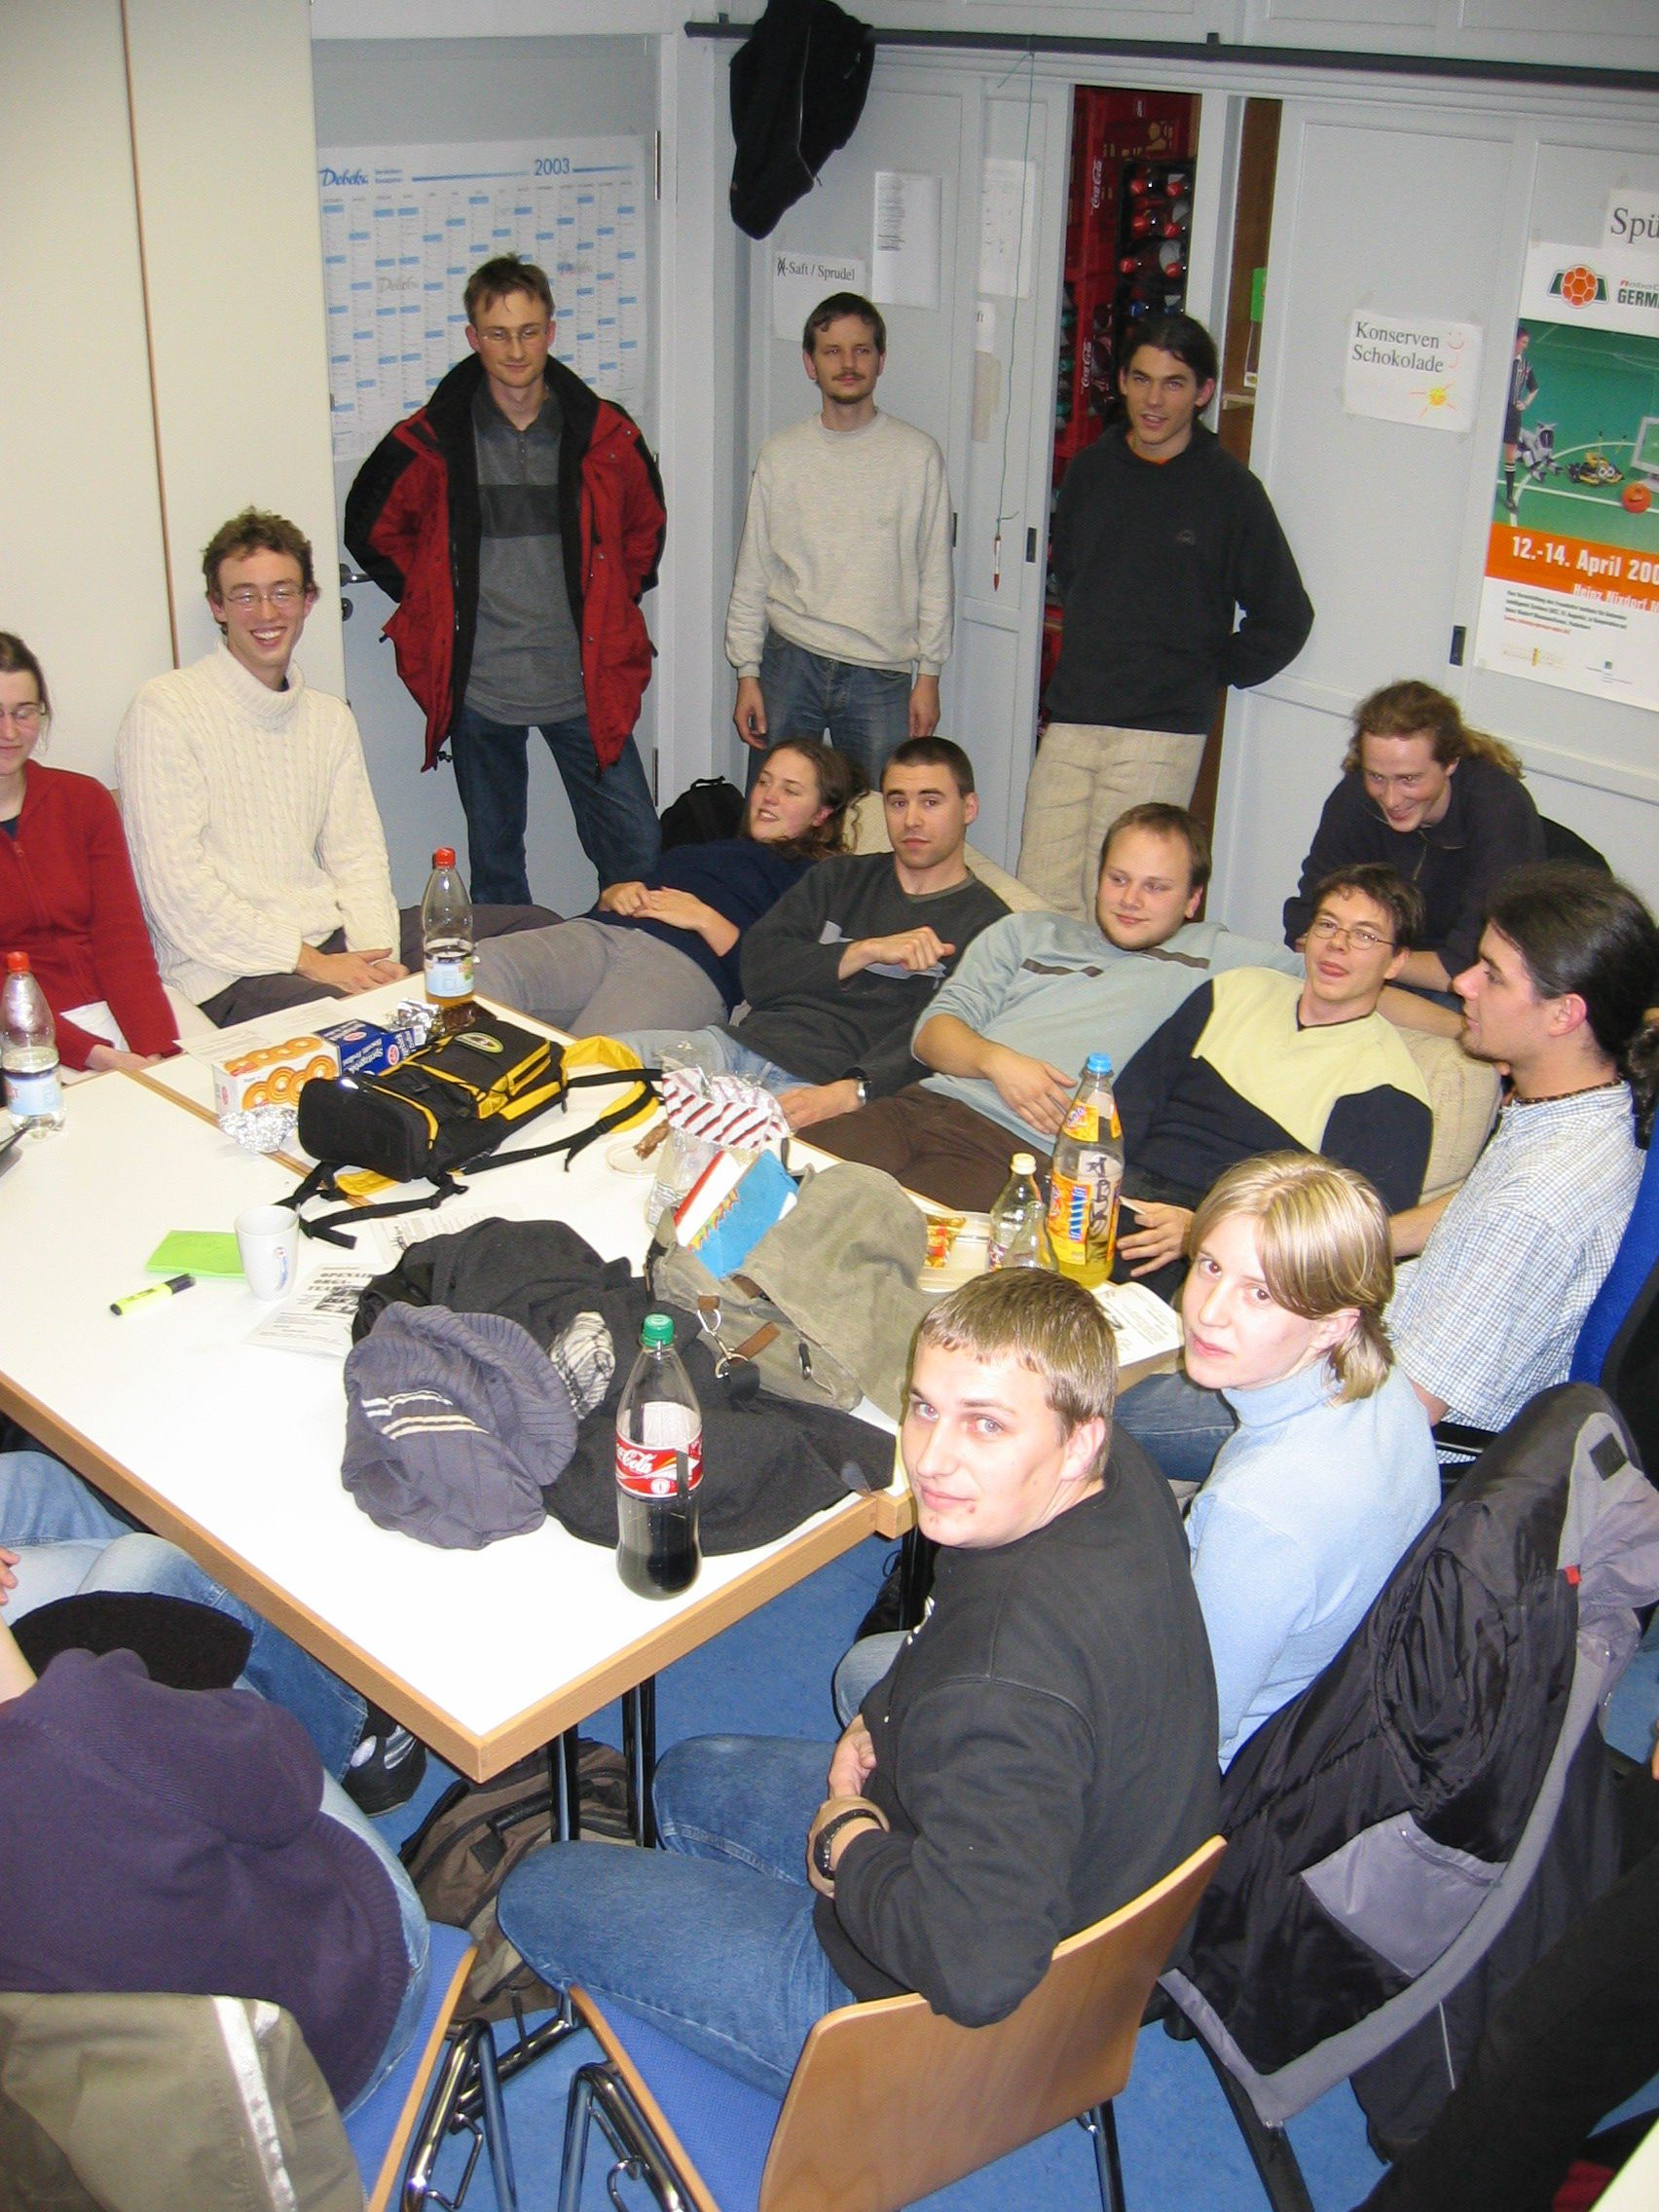
\includegraphics[width=\linewidth]{Sitzung.jpg}
			\end{column}
		\end{columns}
	\end{frame}

	\begin{frame}
		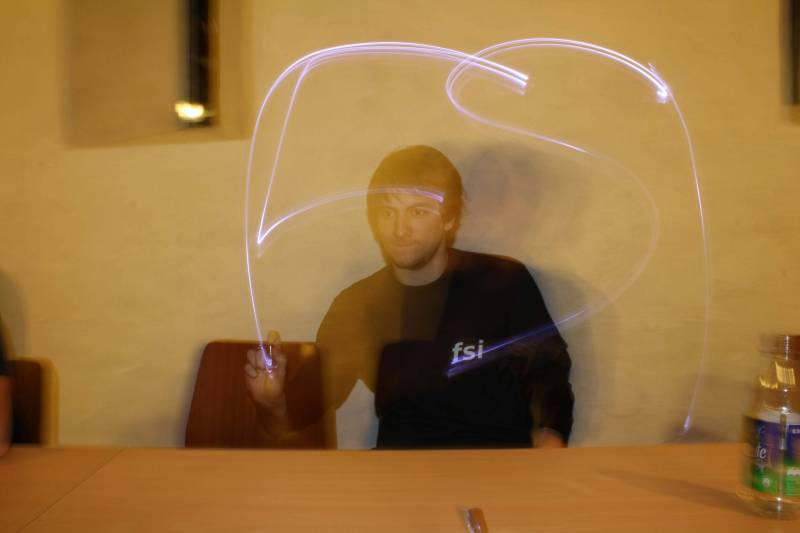
\includegraphics[width=\linewidth]{fsi-manu.png}
		\vspace*{2mm}\\
		{\centering\url{www.fsi.uni-tuebingen.de}}
	\end{frame}
		
	
\end{document}